%>>> Pull plots form algo talks, describe proecess for CC method

%....  get exact equations used for distance ....

%It is clear that OOT pile-up is degrading the time resolution of the ECAL reconstruction. To correct for this we developed the cross correlation method (KUCC) for the timing reconstruction. 
%We will refer to the nine pulses and their pulse amplitudes from the BX before and after the nominal BX as OOT pulses and OOT amplitudes.

The cross correlation method utilizes the ten fitted pulse amplitudes, $A^{mf}_{i}$, derived from the multi-fit method for the energy reconstruction. The actual pulse shape, $H(bx)$, defined by the pulse amplitudes $A^{mf}_{i}$ can be considered to be a linear combination of the nine OOT pulses and the nominal, in-time, pulse of the rechit in a crystal. It is reasonable to say that each of these pulses will arise from a particle incident in the crystal and will therefore exhibit the expected, well-known, characteristic pulse shape produced by a scintillating light burst. It is not reasonable to say that it is known exactly at what location on this expected pulse shape that a particular amplitude, $A^{mf}_{i}$, was measured. 

\begin{figure}[htbp]
\begin{center}
\resizebox{0.95\linewidth}{!}{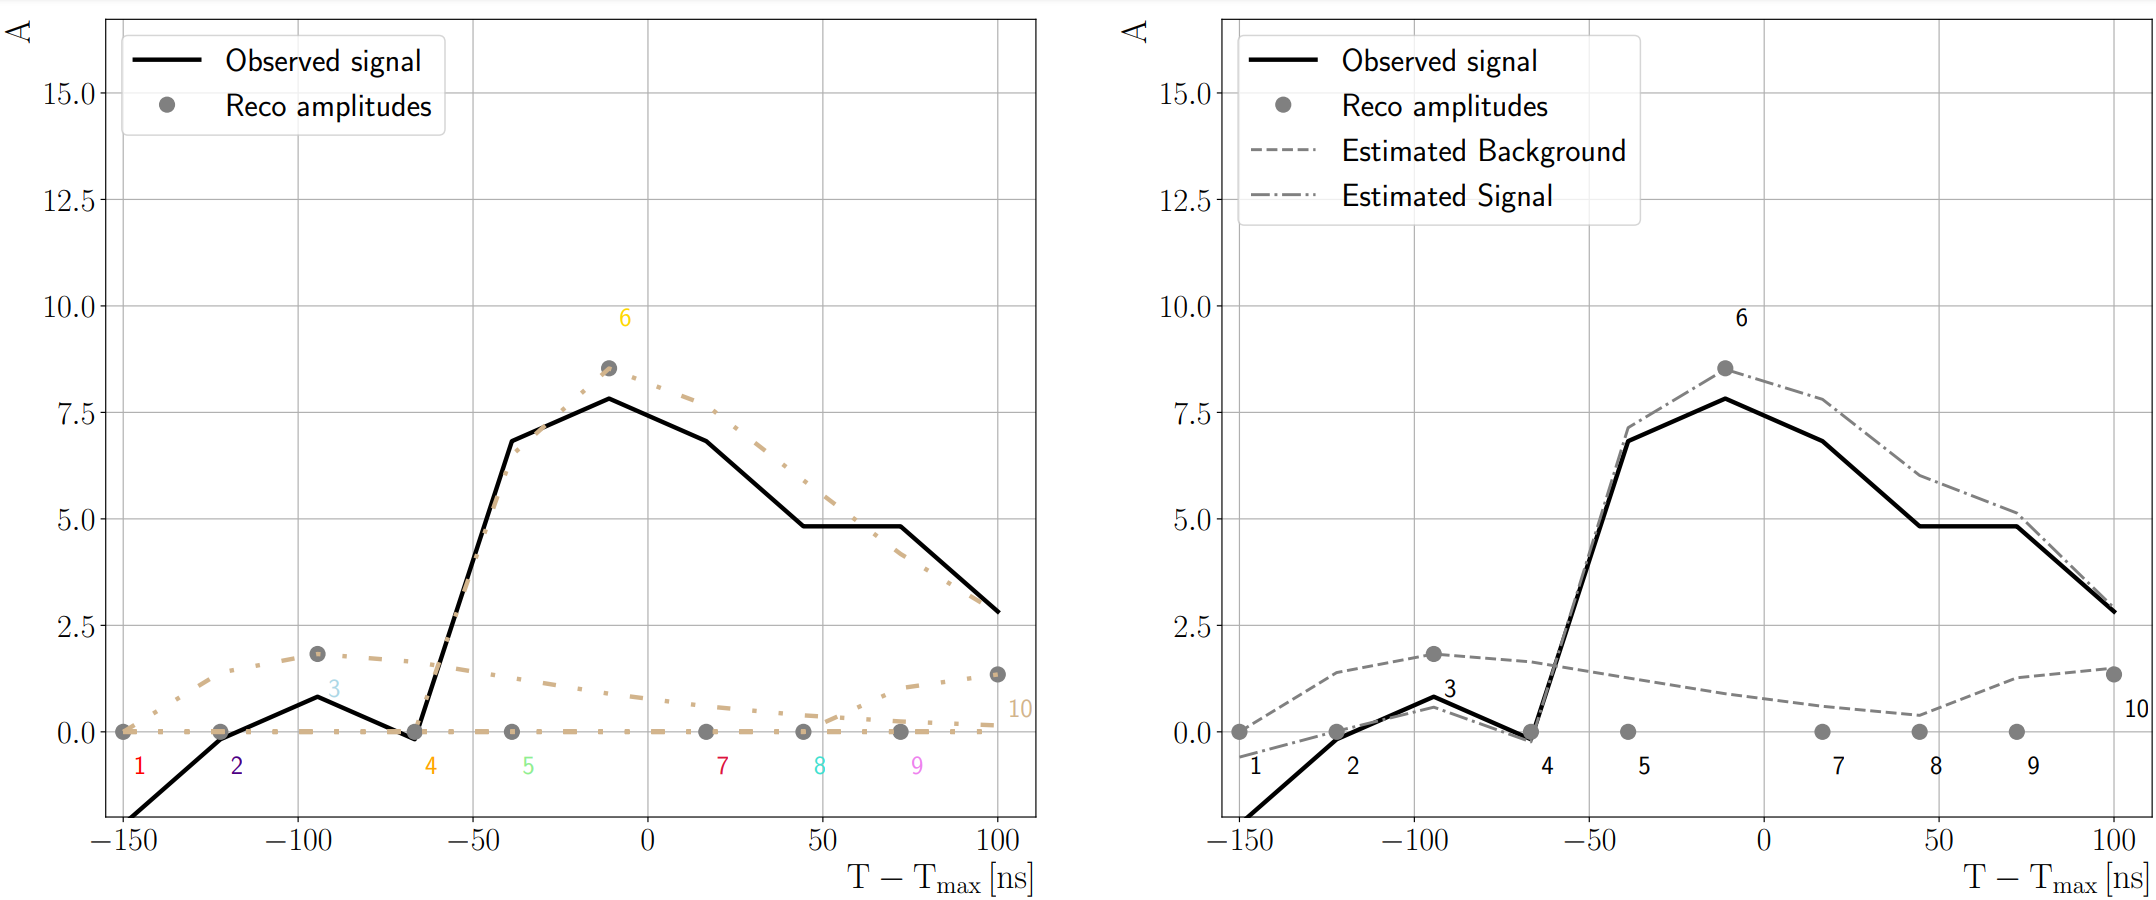
\includegraphics{fig/sec_algos/fOOT_reco_a2.png}}
%\resizebox{0.65\linewidth}{!}{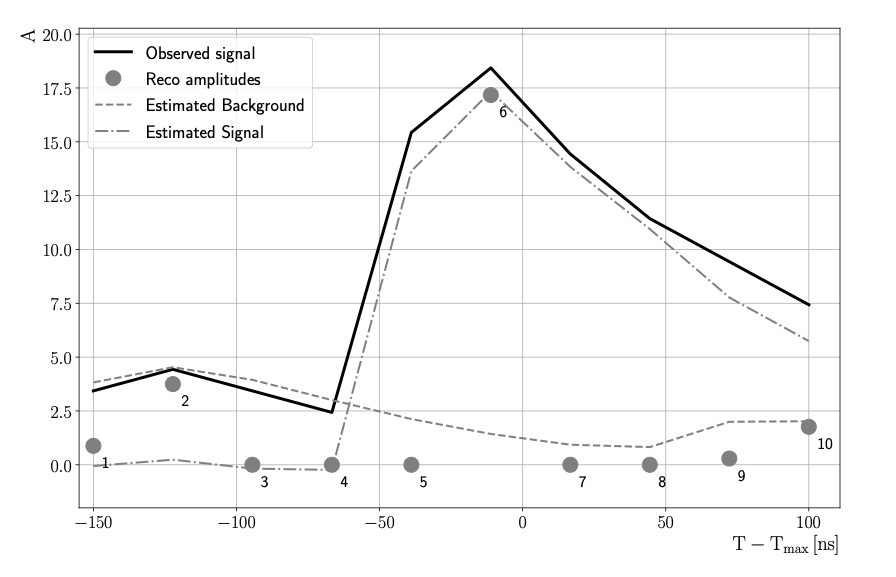
\includegraphics{fig/sec_reco/mfit_pulses_sing.png}}
\caption{An illustration of the OOT amplitude correction for the proposed time reconstruction method. In both plots the black line is the measured signal, $H(bx)$ and the black dots are the reconstructed amplitudes from the multi-fit, $A^{mf}_{i}$. In the plot on the left the double doted dashed lines are the nine OOT pulses, $F^{OOT}_{i}(A^{mf}_{i},t)$, including the nominal, or in-time, pulse given by amplitude 6, that are all reconstructed from $A^{mf}_{i}$. In the plot on the right the dashed line is the background pulse shape, $F_{bg}(bx,t)$, that is the linear combination of the OOT amplitudes. The dotted dashed line is the recovered signal, $A^{sig}(bx,t)$, that is found by subtracting the background pulse shape from the measured signal.}
\label{tra_pulsereco}
\end{center}
\end{figure}

%For this reason we need a continuous function describing the pulse shape so that we can shift the pulse in time.
%We utilize $A^{mf}_{i}$ and the analytic characterization of the pulse shape to define a function, $F^{OOT}_{I}(A^{mf}_{i},t)$, that describes the OOT pulses.
A continuous function describing the characteristic pulse shape is derived with an analytic description that is fit, channel by channel, to the templates of the known characteristic pulse shapes. The amplitudes, $A^{mf}_{i}$, and this analytic description of the characteristic pulse shape is utilized to define a function, $F^{OOT}_{I}(A^{mf}_{i},t)$, that represents the amplitude and time dependence of the shape of the OOT pulses. The sum, or superposition, of the OOT pulses then can be used to define a background pulse shape as given in Equation~\ref{cc_bps}.
\begin{equation}\label{cc_bps}
F_{bg}(bx,t) = \sum F^{OOT}_{i}(A^{mf}_{i},t)\qquad
\end{equation}
As shown in Figure~\ref{tra_pulsereco}, by subtracting $F_{bg}(bx,t)$ from $H(bx)$ we will recover the amplitudes for the nominal pulse which should have the characteristic pulse shape of a scintillating light burst if the correct time parameter for $F^{OOT}_{i}(A^{mf}_{i},t)$ is chosen. Using this approach a signal function, $A^{sig}(bx,t)$, is defined in Equation~\ref{cc_sig} that gives the pulse shape of the in-time, nominal, pulse.  This process is referred to as the OOT amplitude correction.
\begin{equation}\label{cc_sig}
A^{sig}(bx,t) = H(bx) - F_{bg}(bx,t)\qquad
\end{equation}
In both the plots shown in Figure~\ref{tra_pulsereco}, the black lines are the measured signal, $H(bx)$ and the black dots are the amplitudes from the multi-fit, $A^{mf}_{i}$. In the plot on the left the double dotted dashed lines show the nine OOT pulses, $F^{OOT}_{i}(A^{mf}_{i},t)$, that are reconstructed from the amplitudes $A^{mf}_{i}$. In the plot on the right the dotted dashed line is the background pulse shape, $F_{bg}(bx,t)$, as defined in Equation~\ref{cc_bps} and the dashed line is the recovered signal, $A^{sig}(bx,t)$ defined in Equation~\ref{cc_sig}.

\begin{equation}\label{cc_delta}
d(\delta) = (A \star T)(\delta) \equiv \frac{\sum A^{sig}(bx,t)S[bx,\delta]}{\sqrt{\sum (A^{sig}(bx,t)^2 \sum (S[bx,\delta])^2)}}\qquad
\end{equation}

The time of the in-time pulse is determined by finding the time that best matches $A^{sig}(bx,t)$ to the pulse shape template $S[bx]$, where $S[bx]$ is a discrete function of the BX. This is done by constructing a distance, $\delta$, between $A^{sig}(bx,t)$ and the pulse shape template, $S[bx]$, that has a minimum when there is a best overlap between the signal and the template. The time that maximizes the cross correlation function, $d(\delta)$ given in Equation~\ref{cc_delta}, is then the reconstructed time for a rechit in a crystal. This second step is referred to as the cross correlation fit.

In the case where the reconstructed time is delayed more than $\sim$1 ns, the OOT amplitude correction returns a biased result that tends to underestimate the reconstructed time by a factor of two. This effect is discussed in the next section, Section~\ref{sec:recobias}. 

%from a weighted $\chi^{2}$ function : 
%$$D = \sum_{bx} (A^{sig}(bx,t) - S[bx])^{2}|A^{sig}(bx,t) \times S[bx]|\qquad(9)$$


